\documentclass{article}

\usepackage{amsmath, amsthm, amssymb, amsfonts}
\usepackage{thmtools}
\usepackage{graphicx}
\usepackage{setspace}
\usepackage{geometry}
\usepackage{float}
\usepackage{hyperref}
\usepackage[utf8]{inputenc}
\usepackage[english]{babel}
\usepackage{framed}
\usepackage[dvipsnames]{xcolor}
\usepackage{tcolorbox}
\usepackage{dcolumn}
\usepackage{indentfirst}

\colorlet{LightGray}{White!90!Periwinkle}
\colorlet{LightOrange}{Orange!15}
\colorlet{LightGreen}{Green!15}

\newcommand{\HRule}[1]{\rule{\linewidth}{#1}}

\declaretheoremstyle[name=Theorem,]{thmsty}
\declaretheorem[style=thmsty,numberwithin=section]{theorem}
\tcolorboxenvironment{theorem}{colback=LightGray}

\declaretheoremstyle[name=Proposition,]{prosty}
\declaretheorem[style=prosty,numberlike=theorem]{proposition}
\tcolorboxenvironment{proposition}{colback=LightOrange}

\declaretheoremstyle[name=Principle,]{prcpsty}
\declaretheorem[style=prcpsty,numberlike=theorem]{principle}
\tcolorboxenvironment{principle}{colback=LightGreen}

\setstretch{1.2}
\geometry{
    textheight=9in,
    textwidth=5.5in,
    top=1in,
    headheight=12pt,
    headsep=25pt,
    footskip=30pt
}

% ------------------------------------------------------------------------------

\begin{document}

% ------------------------------------------------------------------------------
% Cover Page and ToC
% ------------------------------------------------------------------------------

\title{ \normalsize \textsc{}
		\\ [2.0cm]
		\HRule{1.5pt} \\
		\LARGE \textbf{\uppercase{US Inflation Hedge Strategies}
		\HRule{1.5pt} \\ [0.6cm] \LARGE{Digital Tools For Finance} \vspace*{10\baselineskip}}
		}
\date{December 18, 2023}
\author{\textbf{Andreas Pozzi 23-715-923} \\ 
\textbf{Zhiyu Wei 23-744-576} \\ 
\textbf{Diana Jin 23-714-082} \\ 
\textbf{Hanieh Jebeli 23-744-014} \\ 
		%Where? \\
		%When?
  }

\maketitle
\newpage

\tableofcontents
\newpage

% ------------------------------------------------------------------------------
\begin{abstract}
Inflation is a natural occurrence in the market economy, and it is important to find the right strategies and investments to hedge against it. It increases the prices of goods and services which thus diminishes investment returns, prompting investors to seek hedges against the consequent devaluation of their assets. In our research, we explore the hedging qualities of various domestic assets available to US investors to find the best asset to use against inflation. Using monthly values of the Consumer Price Index (CPI) and prices of the S\&P500, the iShares TIPS Bond ETF, the Vanguard Real Estate Index Fund, and gold (via the London bullion benchmark) from January 2004 to October 2023, we employed a simple linear regression under the assumptions of symmetry and no time-variance to measure inflation hedging properties. Our findings indicate the Vanguard Real Estate Index Fund as the superior hedge, followed by gold and the S\&P500, although robustness checks suggest limitations in the model's suitability.
\end{abstract}

% ------------------------------------------------------------------------------
\section{Introduction} Inflation is a general increase of the prices of goods and services in an economy, typically measured by the Consumer Price Index (CPI). During investment activities, the aim of a rational investor is to maximize returns and reduce risk. However, inflation has been found to have a negative effect on this aim, as inflation causes a potential reduction in returns on investment assets. By hedging against inflation, the investor protects themselves from a decrease in purchasing power of a currency that results from the loss of its value due to rising prices. Therefore, looking for a good inflation hedge is meaningful for investors. Our analysis aims to calculate the beta coefficient for various asset classes to evaluate their performance as inflation hedges. This involves a regression analysis where the asset returns are regressed against inflation rates to understand the extent of their correlation and to quantify the hedging capability of each asset class. This analysis is grounded in the Fisher Hypothesis, initially proposed by Fisher in 1930 \cite{fisher1930theory}, which establishes a theoretical framework for understanding the relationship between asset returns and inflation. This hypothesis suggests that nominal interest rates are a combination of real returns and the inflation rate. Extending this idea, Fama and Schwert \cite{FAMA1977115} and later Arnold and Auer \cite{ARNOLD2015187} argue that expected nominal returns across various assets are indicative of market expectations about inflation rates.

% ------------------------------------------------------------------------------
\section{Data}
There are many ways to hedge against inflation; a disciplined investor can plan for inflation by investing in asset classes that outperform the market during inflationary climates. Some of the most common anti-inflation assets include gold, commodities, various real estate investments, and TIPS (Treasury Inflation-Protected Securities). In our research, we analyze commonly used assets to hedge against inflation, namely securities and gold, and take the US Consumer Price Index data to calculate inflation values.

\subsection{Gold}
There are several ways to invest in gold, including buying physical gold bars or coins and purchasing exchange-traded funds (ETFs) or mutual funds that track the price of gold, allowing access to gold features and options. Investing in gold mining companies is another way to gain exposure to gold. These companies' share prices do not track gold's value very well over the long run, but they can provide a way to invest in gold indirectly \cite{investopediaInvestGold}. Gold is often used as an investment asset to hedge against inflation and political unrest because of its low correlation with other asset classes \cite{investopediaAssetClasses}. Moreover, it is considered a safe haven asset, which means that it is expected to retain its value or even increase in value during times of economic uncertainty \cite{key}.
We used London Bullion Market benchmark gold prices provided by Nasdaq to source gold market prices analyzed in the regression.

\subsection{Securities}
Securities is an asset class that is commonly used by commercial enterprises use to raise new capital and can be broadly categorized into debts, equities and derivatives \cite{wikipediaSecurityfinance}.  
\\~\\
Debt securities may be called debentures, bonds, deposits, notes or commercial paper depending on their maturity, collateral and other characteristics. The holder of a debt security is typically entitled to the payment of principal and interest, together with other contractual rights under the terms of the issue, such as the right to receive certain information. Debt securities are generally issued for a fixed term and redeemable by the issuer at the end of that term. Equities are shares of ownership in a company. Buying a stock means becoming a shareholder of the company and having a claim on a portion of the company's assets and earnings. Investors can buy and sell equities to make a profit, and they can also receive dividends, which are a portion of the company's profits paid out to shareholders. 
\\~\\
Equities are considered a high-risk, high-reward investment because their prices can be volatile, and profits uncertain. However, over the long term, equities have historically provided higher returns than other asset classes, such as bonds or cash \cite{smartassetWhatEquities}. There are many different types of equity, including common stock, preferred stock, and exchange-traded funds (ETFs). Common stock is the most common type of equity, and it represents ownership in a company with voting rights and the potential for dividends. Preferred stock is a type of equity that has a higher claim on a company's assets and earnings than common stock but does not have voting rights. ETFs are a type of equity that tracks a basket of stocks and can be bought and sold like a stock.

\subsubsection{S\&P500 Index (\textasciicircum{}GSPC)}
The S\&P500 Index, or Standard\&Poor's 500 Index, is a market-capitalization-weighted index of 500 leading publicly traded companies in the U.S. It is widely regarded as a gauge of large-cap U.S. equities, including 500 leading companies and covering approximately 80\% of available market capitalization. The index uses a market-cap weighting method, giving a higher percentage allocation to companies with the largest market capitalizations \cite{S&P500}. The S\&P 500 is often used as a benchmark for the overall stock market performance, and investors use it to compare the risks and returns of other investments. For the scope of our research, the S\&P500 data from Yahoo Finance will be analyzed.

\subsubsection{iShares TIPS Bond ETF (TIP)}
The iShares TIPS Bond ETF seeks to track the investment results of an index composed of inflation-protected U.S. Treasury bonds. Treasury Inflation-Protected Securities \cite{investopediaTreasuryInflationProtected} are a type of treasury security issued by the U.S. government. TIPS are indexed to inflation to protect investors from a decline in the purchasing power of their money. 

\subsubsection{Vanguard Real Estate ETF (VNQ)}
The VNQ ETF, also known as the Vanguard Real Estate ETF, is a popular investment option that falls under the category of real estate investment trusts (REITs \cite{etfinsiderWhat}). As an ETF, it is traded on stock exchanges, providing investors with an opportunity to gain exposure to the real estate market without having to invest directly in individual properties. VNQ is designed to track the performance of the MSCI US Investable Market Real Estate 25/50 Index, a benchmark that includes various REITs in the United States. 

\subsection{Consumer Price Index}
The Consumer Price Index (CPI) is a measure of the average change over time in the prices paid by urban consumers for a market basket of consumer goods and services \cite{blsHomeUS}. It is widely regarded as a gauge of inflation and deflation in the U.S. economy. The CPI is calculated by the Bureau of Labor Statistics and is based on data collected from thousands of households across the country. The CPI is used by policymakers, economists, and investors to track inflation and make decisions about monetary policy, fiscal policy, and investment strategies.
For the purpose of the project, the inflation will be accounted for using the CPI data published regularly by the US Bureau of Labor Statistics.

% ------------------------------------------------------------------------------
\section{Methodology}
\subsection{Theoretical Model}
The inflation hedge of any asset class is usually predicated on the Fisher hypothesis, which renders the first attempt to formally state the hypothetical relationship between asset returns and inflation. Under this hypothesis, the nominal interest rate is expressed as the sum of real returns and inflation rate. Therefore, real returns fall as inflation rate increases, unless nominal interest rates increase at the same rate as inflation. That is to say, the definition of hedging against inflation is that the expected nominal interest rate should move in sync with expected inflation. Thus, we can specify a generalized Fisher hypothesis framework for the inflation hedging of a particular asset class as follows:
\begin{center}
{\(r_t = \alpha + \beta \pi_t + \epsilon_t; \quad \epsilon_t \sim N(0, \sigma^2_{\epsilon})\)}.
\end{center}
\(r_t\) is the asset return at period $t$ given as 
\begin{equation*}
    r_t = 100*\log\left(\frac{p_t}{p_{t-1}}\right),
\end{equation*} 
where $p$ denotes the price of the asset, and $\pi_t$ is the inflation rate at period $t$ given as 
\begin{equation*}
   \pi_t = 100*\log\left(\frac{cpi_t}{cpi_{t-1}}\right),
\end{equation*}
where $cpi$ denotes the Consumer Price Index value. \\~\\
Thus, the coefficient \(\beta\) is a measurement of the inflation hedge, where
\begin{align*}
    \beta &= 0 \text{ means the asset has no inflation hedging potential;}\\
    0 < \beta &< 1 \text{ means the asset partially hedges against inflation;} \\
    \beta &=1 \text{ means that the asset is fully hedging against inflation;} \\
    \beta &>1 \text{means that the asset has superior hedging performance.}
\end{align*}

\subsubsection{Assumptions of the Model}
\noindent
\textbf{Symmetry} \\
\indent
We assume that the relationship between the asset price and inflation is symmetric, which means the differences in the asset's ability to hedge are ignored, regardless of whether there are positive or negative changes in inflation.\\~\\
\textbf{No Time-Variance} \\
\indent 
Although previous research has pointed out that the inflation hedging potential of some assets individually could be time-varying (e.g. it may show high reaction to structural changes in the economy, or may function as a hedge against inflation only in specific economic conditions or data ranges), to simplify our model, we assume that the hedging potential of the asset in question computed by the Fisher model can represent its average ability to hedge.

% ------------------------------------------------------------------------------
\subsection{Implementation}
Using APIs provided by the US Bureau of Labor Statistics and Nasdaq Data Link, as well as the \verb|yfinance| Python API for Yahoo Finance, we pulled monthly asset prices and CPI values and appended the data into CSV files. We then calculated monthly returns and implemented our regression model. After running the regression model, we performed robustness checks to ensure the reliability and validity of the analysis through cross-validation and running a robust regression (i.e. Huber regression). We then analyzed the results to find the asset with the best hedging performance.
\\~\\
The time period analyzed in our model is from 01.01.2004 to 31.10.2023. We provide instructions and fully replicable code on the GitHub repository \footnote{Repository: {\href{https://github.com/dianayjin/US-inflation-hedge-strategies}{US-inflation-hedge-strategies}}.}.

% ------------------------------------------------------------------------------
\section{Results}
\subsection{Regression Model}
The results obtained from our regression model have highlighted different levels of inflation hedging among the strategies analyzed (Table \ref{tab:regtable}). VNQ (Vanguard Real Estate Investment Fund ETF) has a beta coefficient higher than one, indicating superior hedge performance and making it the best strategy among the ones considered. Both gold and \textasciicircum{}GSPC are partial hedges, with a beta coefficient of about 0.5, meaning that these instruments are only partially able to insulate against inflation. TIP is shown to be the worse instrument to hedge inflation. With a regression beta coefficient of less than zero, TIPs have no hedging potential and have returns that are very sensitive to inflation fluctuations.

\newcolumntype{d}[1]{D{.}{.}{#1}}
\begin{table}[h!]
  \centering
  \begin{tabular}{|c|d{4.4}|d{4.4}|c|c|}
    \hline
    \textbf{Asset Name} & \multicolumn{1}{c|}{\textbf{$\beta$ Coefficient}} & \multicolumn{1}{c|}{\textbf{Intercept}} & \multicolumn{1}{c|}{\textbf{MSE}} & \multicolumn{1}{c|}{\textbf{COD (R\textsuperscript{2} Score)}} \\
    \hline
    Gold & 0.5658 & 0.0059 & 0.0024 & 0.0022 \\
    \hline
    TIP & -0.0985 & 0.0029 & 0.0003 & 0.0005 \\
    \hline
    VNQ & 1.1018 & 0.0032 & 0.0044 & 0.0046 \\
    \hline
    \textasciicircum GSPC & 0.5291 & 0.0046 & 0.0019 & 0.0024 \\
    \hline
  \end{tabular}
  \caption{Regression results.}
  \label{tab:regtable}
\end{table}
\begin{figure}[H]
    \centering
    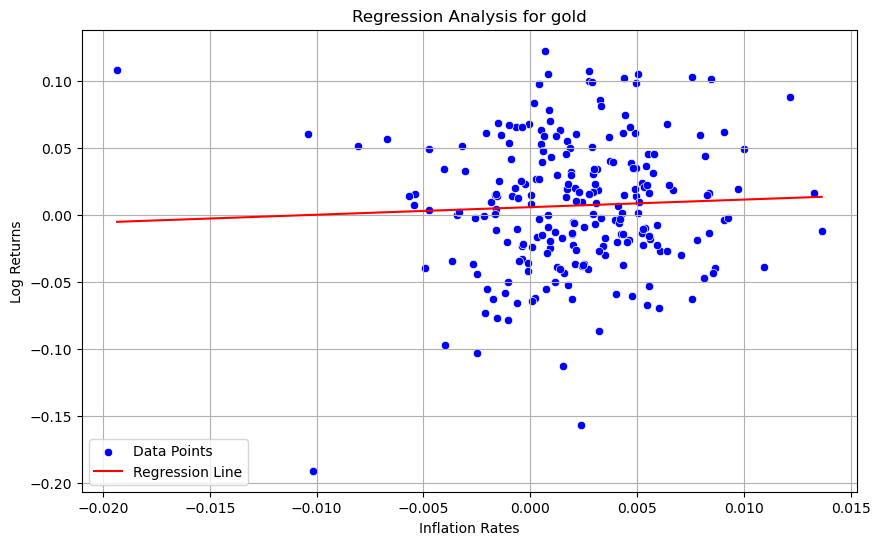
\includegraphics[width=0.75\linewidth]{reports\figures\Regressionanalysisforgold.png}
    \caption{Regression table for gold returns.}
\end{figure}
\begin{figure}[H]
    \centering
    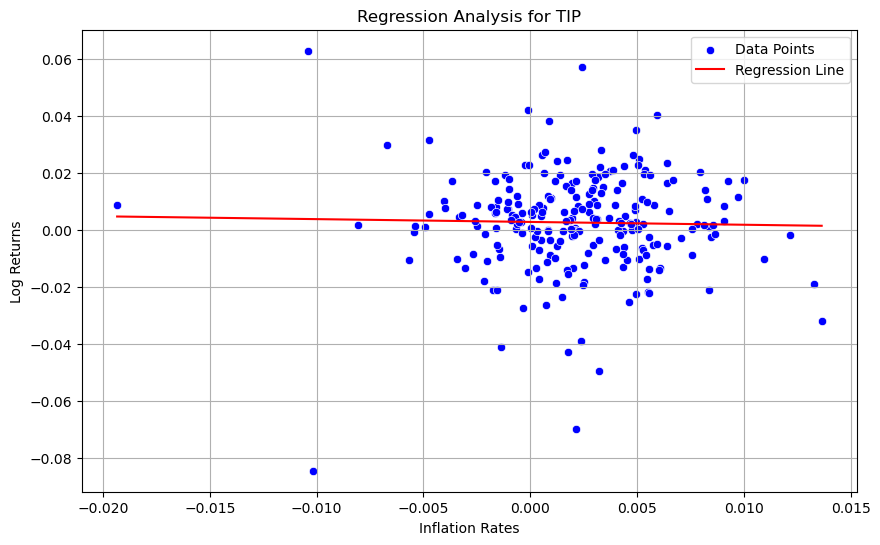
\includegraphics[width=0.75\linewidth]{reports\figures\RegressionanalysisforTIP.png}
    \caption{Regression table for iShares TIPS Bond returns.}
\end{figure}
\begin{figure}[H]
    \centering
    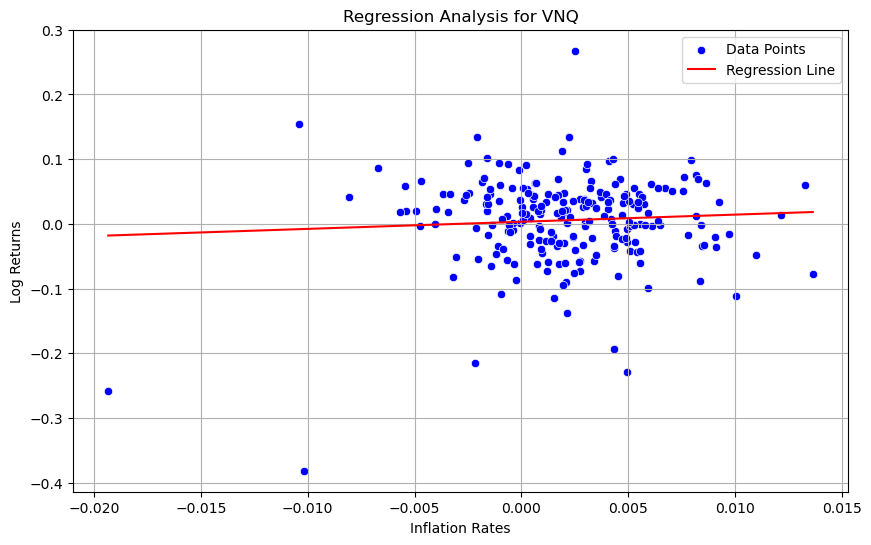
\includegraphics[width=0.75\linewidth]{reports\figures\RegressionanalysisforVNQ.png}
    \caption{Regression table for Vanguard Real Estate Index Fund returns.}
\end{figure}
\begin{figure}[H]
    \centering
    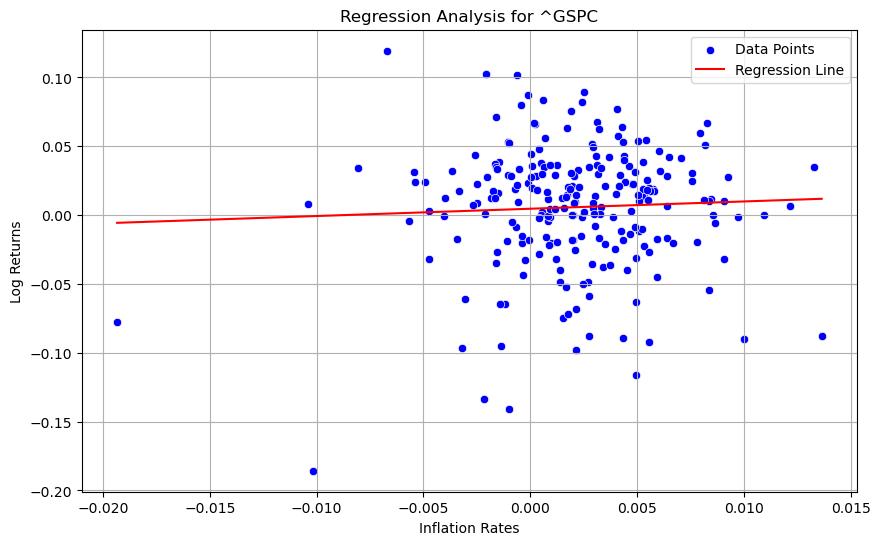
\includegraphics[width=0.75\linewidth]{reports\figures\RegressionanalysisforGSPC.png}
    \caption{Regression table for S\&P500 Index returns.}
\end{figure}

\subsection{Robustness Checks}
Performing a robustness check on a regression model typically involves testing how well the model holds up under various conditions or assumptions. Common methods for robustness checks include cross-validation, which tests the model's performance on different subsets of the data; adding/removing variables, which assesses the impact of adding or removing explanatory variables; using different time periods, which tests the model on different time periods to see if it maintains its predictive power; robust regression methods, which employs regression techniques that are less sensitive to outliers, such as RANSAC, Theil-Sen, or Huber regressions. To test our model for robustness, we used cross-validation and implemented a Huber regression.

\subsubsection{Cross-Validation}
Cross-validation is a way to predict the fit of a model to a hypothetical validation set when an explicit set is not available. Ideally, low variance and low bias suggest that the model generalizes well from the training data to unseen data. \(R^2\) is a statistical measure that represents the proportion of the variance for the dependent variable that's explained by the independent variables in a regression model. To interpret our cross-validation results, for an \(R^2\) score close to 1 implies that the model performed very well on the corresponding data set, explaining a large portion of the variance; if the \(R^2\) score is positive but far from 1, the model has some predictive ability but is not as robust; if the \(R^2\) score is 0, the model's predictions are no better than a random guess; if the \(R^2\) score is negative, the model's predictions are worse than a simple model based on the mean of the data.
\\~\\
In our analysis, we use 5-fold  cross-validation; the results are shown in the chart below (Table \ref{tab:table1}). From the results, the average \(R^2\) scores for four assets are all negative, which implies the model is not appropriate for the data. This is mainly because we only use simple linear regression model to analyze the relation between inflation and returns of assets, relying on strong assumptions that are not observed in reality.

\begin{table}[h!]
  \centering
  \begin{tabular}{|c|c|c|}
    \hline
    \textbf{Asset Name}  &  \textbf{CV Average R\textsuperscript{2}} & \textbf{CV R\textsuperscript{2} Scores} \\
    \hline
    Gold & -0.0219 & [-0.0090, -0.0028, 0.0033, -0.0040, -0.0968] \\
    \hline
    TIP & -0.0574 & [-0.0151, -0.1226, 0.0008, -0.1230, -0.0272] \\
    \hline
    VNQ & -0.0260 & [-0.0687, -0.0253, -0.0436, 0.0065, 0.0009] \\
    \hline
    \textasciicircum GSPC & -0.1228 & [-0.2961, -0.0841, -0.0276, -0.0710, -0.1354] \\
    \hline
  \end{tabular}
  \caption{Cross validation robustness check results.}
  \label{tab:table1}
\end{table}

\subsubsection{Huber Regression}
Huber regression combines the attributes of the OLS regression and median regression to provide a model that is more robust against outliers. The interpretation of Huber regression results is similar to interpreting standard regression coefficients, and coefficients in Huber regression are generally more robust and reliable in the presence of outliers.
\\~\\
The results of the Huber regression is shown in the graph below (Table \ref{tab:table2}). The beta coefficients for gold, TIP, and VNQ are all negative, showing no hedging potential. The coefficient for \textasciicircum GSCP is 0.0006,  which is very close to zero, indicating a very weak hedging potential. 

\begin{table}[h!]
  \centering
  \begin{tabular}{|c|D{.}{.}{4.4}|D{.}{.}{4.4}|}
    \hline
    \textbf{Asset Name} & \multicolumn{1}{c|}{\textbf{Robust $\beta$ Coefficient}} & \multicolumn{1}{c|}{\textbf{Robust Intercept}} \\
    \hline
    Gold & -0.2691 & 0.0076\\
    \hline
    TIP & -0.1579 & 0.0038\\
    \hline
    VNQ & -1.1747 & 0.0138\\
    \hline
    \textasciicircum GSPC & 0.0006 & 0.0101\\
    \hline
  \end{tabular}
  \caption{Huber robustness check results.}
  \label{tab:table2}
\end{table}
% ------------------------------------------------------------------------------


% Reference and Cited Works
% ------------------------------------------------------------------------------
%This is a citation\cite{Eg}.

\newpage
\bibliographystyle{IEEEtran}
\bibliography{references.bib}

% ------------------------------------------------------------------------------

%\begin{theorem}
    %This is a theorem.
%\end{theorem}

%\begin{proposition}
    %This is a proposition.
%\end{proposition}

%\begin{principle}
    %This is a principle.
%\end{principle}

% Maybe I need to add one more part: Examples.
% Set style and colour later.

%\subsection{Pictures}

%\begin{figure}[htbp]
    %\center
    %\includegraphics[scale=0.06]{img/photo.jpg}
    %\caption{Sydney, NSW}
%\end{figure}

%\subsection{Citation}



%\newpage

\end{document}
